%! TEX root = ../main.tex
\documentclass[../main.tex]{subfiles}
\begin{document}
\section{Anwendungen in Forschung und Industrie}
\begin{figure}[H]
	\centering
	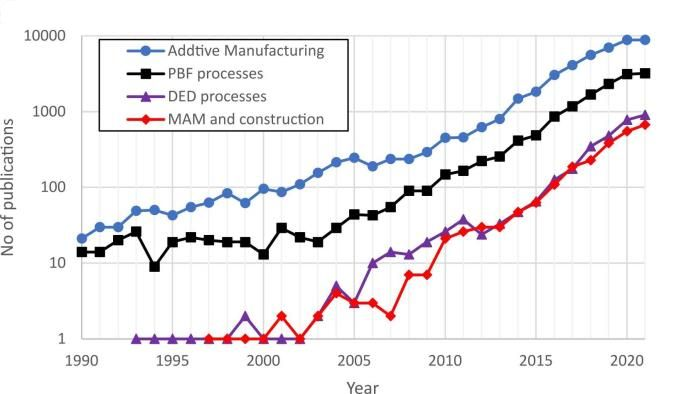
\includegraphics[width=1\textwidth]{search5}
	\ccaption{Anzahl an wissenschaftlichen Artikeln und Publikationen zum Thema 3D-Druck}{adaptierte Grafik, von \protect\cite{KANYILMAZ2022102541} entnommen}
	\label{img:search_5}
\end{figure}
Wie aus Abb. \ref{img:search_5} erkennbar ist, ist die Nachfrage und Forschung für die Anwendung des 3D-Drucks, besonders für die \acrlong{slm}- und \acrfull{pbf}-Prozesse, stark angestiegen in den letzten beiden Jahrzehnten.

\begin{figure}[H]
	\centering
	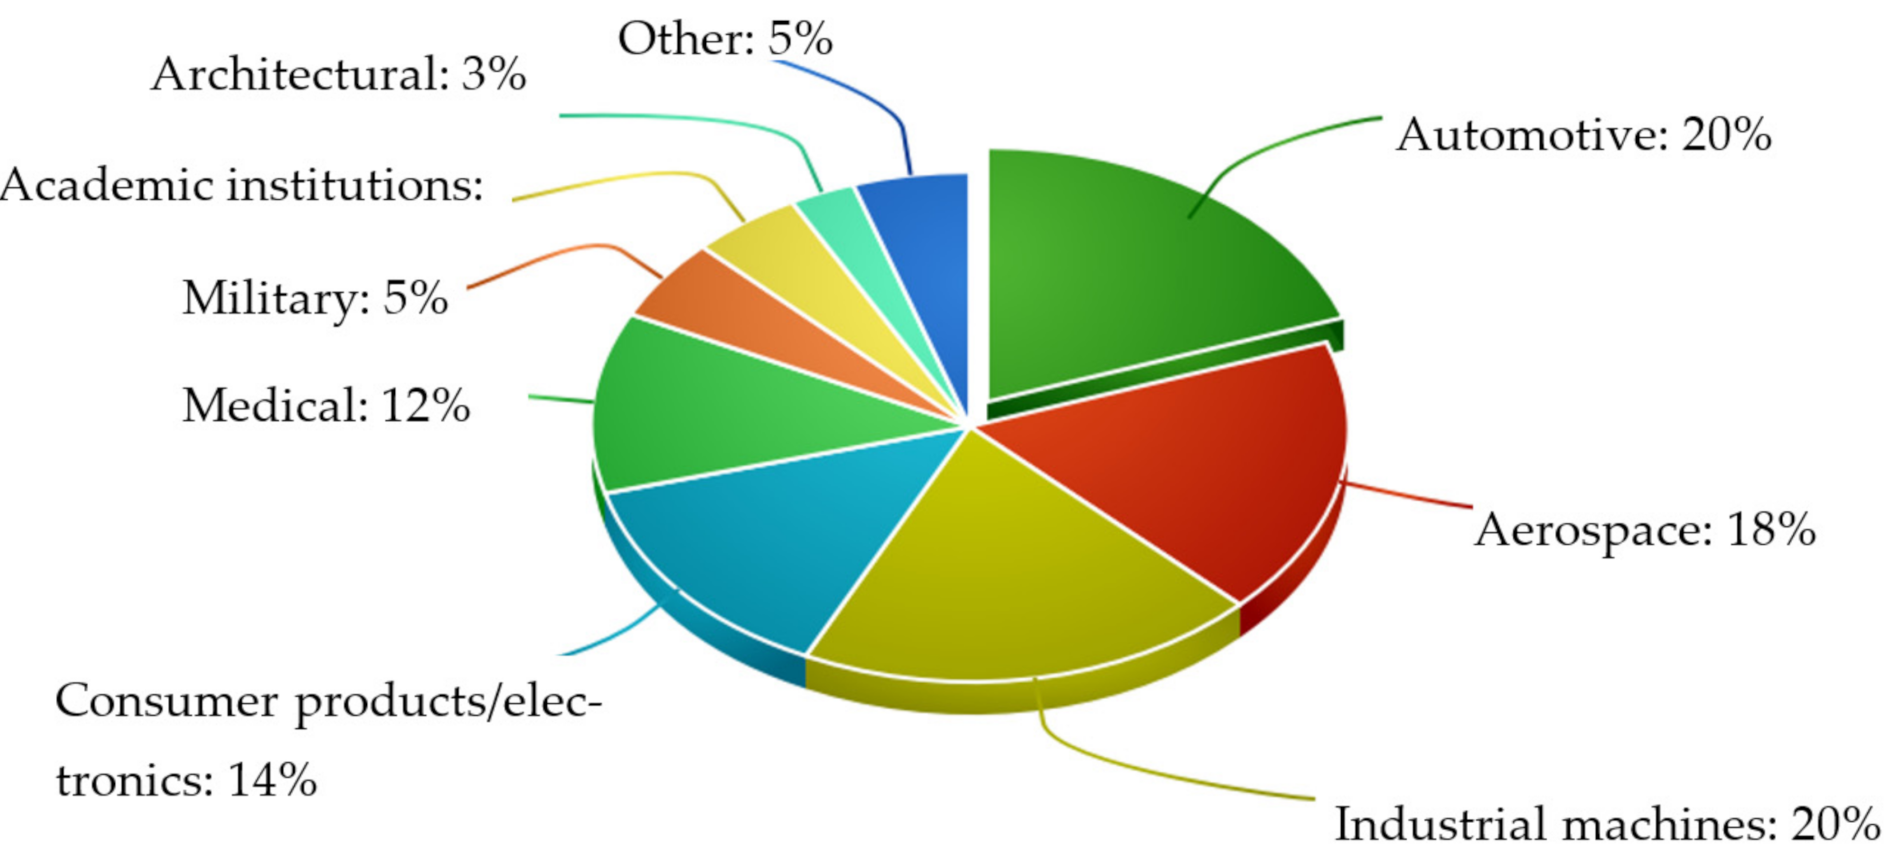
\includegraphics[width=1\textwidth]{am_shares}
	\ccaption{Anteile verschiedener Anwendungsgebiete im \acrshort{am} (Stand 2017)}{Grafik von \protect\cite{app11031213} entnommen}
	\label{img:am_shares}
\end{figure} 
\subsection{Forschung}
\subsection{Industrie}
\subsubsection{Reparatur und OOP-Ersatzteil-Produktion}
%Dies ist besonders praktisch für Firmen, welche auf alte Maschinen angewiesen sind, deren Ersatzteile schon längst außer Produktion sind. Die Anschaffungskosten eines Metall-3D-gedruckten Werkstückes sind zwar enorm hoch, aber dennoch günstiger in vielen Fällen als das Produkt substraktiv herzustellen.
\subsubsection{Leichtbauindustrie}

\end{document}
